\handsonEnv
%%%
\begin{frame}
\frametitle{\href{https://wci.llnl.gov/simulation/computer-codes/visit/}{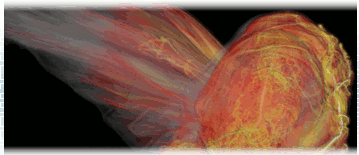
\includegraphics[height=.85cm]{figs/visit-logos/VisIt-03}} \hspace{-.85cm}{\bf \textcolor{lightgray}{VisIt}}: Intermesso i}

\begin{beamerboxesrounded}[upper=block head,lower=block body,shadow=true]{\bf Hands-on...}%Assignment ii}
%        \textcolor{DarkRed}{\ding{231}} try loading some of the datasets we used with ParaView [{\small \textcolor{gray}{\tt headsq.vtk}, \textcolor{gray}{\tt testRectilinearGrid.vtk}, \textcolor{gray}{\tt disk\_out\_ref.ex2}, ...}] --or-- your own data!!!
        \textcolor{DarkGreen}{\ding{231}} Load some of the other datasets: 
                [eg. {\small "\textcolor{gray}{\texttt{testRectilinearGrid.vtk}}", "\textcolor{gray}{\texttt{headsq.vtk}}", "\textcolor{gray}{\texttt{disk\_out\_ref.ex2}}", ...}]
                --or-- \textit{your own data}!!!

        \pause
        \textcolor{DarkGreen}{\ding{231}} Try to explore the data and visualize it, using some of the tools we have discussed

	\pause
        \textcolor{DarkGreen}{\ding{231}} If you have used other visualization packages, compare how easy and 
                whether it is possible or not, to obtain similar results, let's say, with ParaView or VAPOR for instance...

        \textcolor{DarkGreen}{\ding{231}} also which one, results more intuitive, elegant, useful for you and your research
\end{beamerboxesrounded}

\pause
\vspace{2mm}
\begin{columns}
\begin{column}{3cm}
	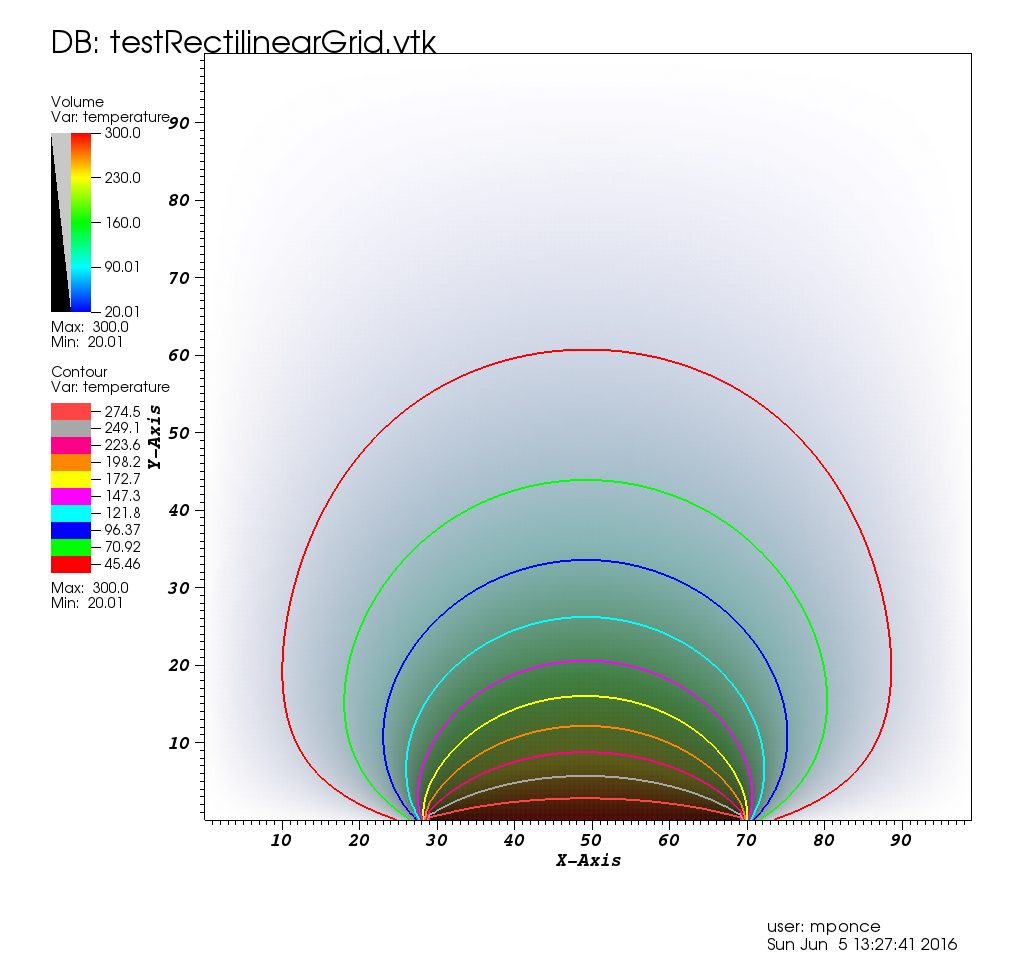
\includegraphics[width=.9\columnwidth]{figs/visit-handson/testRectilinearGrid}
\end{column}
\begin{column}{3cm}
	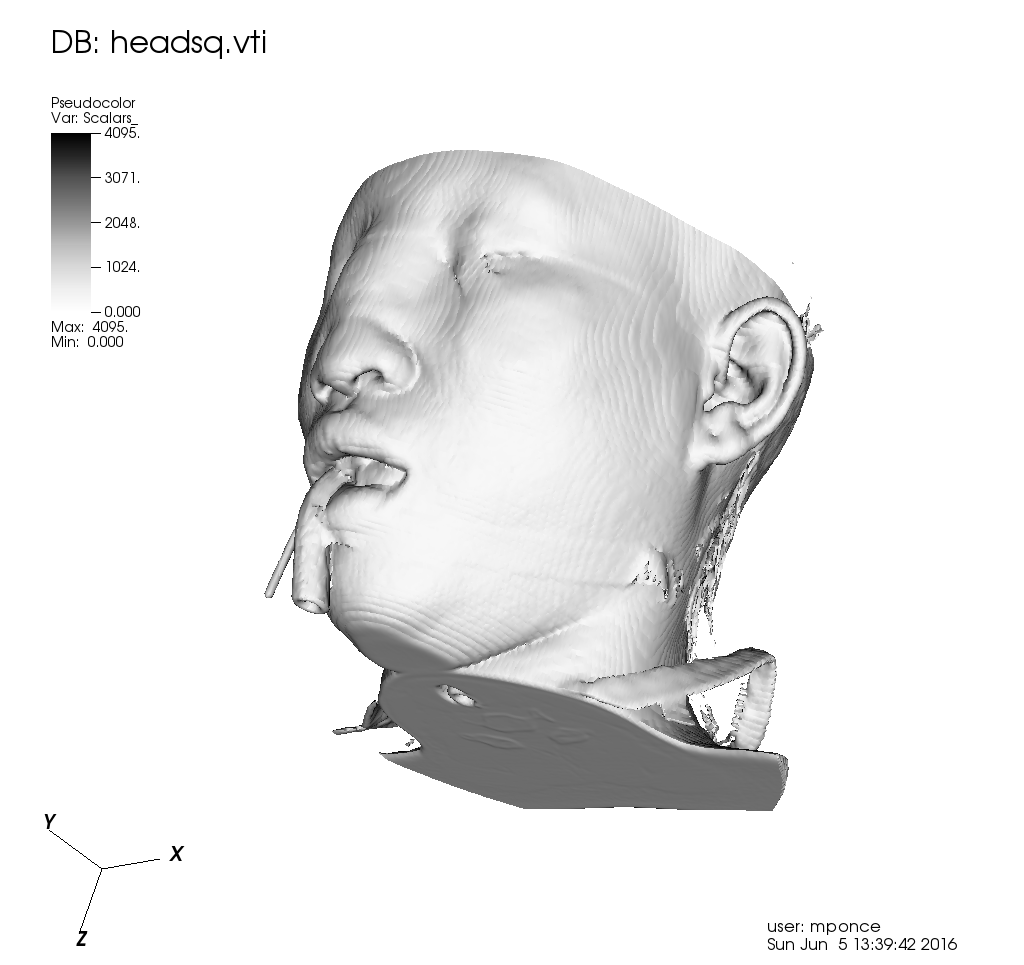
\includegraphics[width=.9\columnwidth]{figs/visit-handson/headsq}
\end{column}
\begin{column}{3cm}
	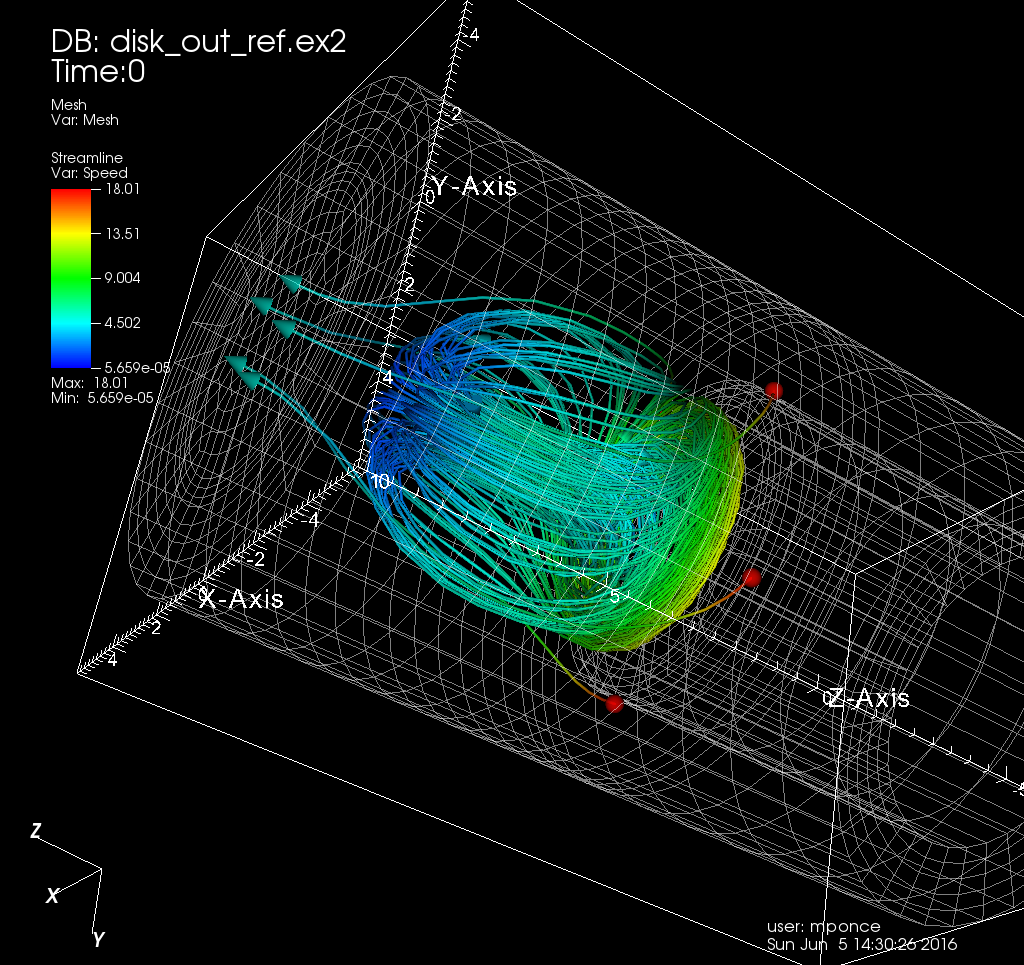
\includegraphics[width=.9\columnwidth]{figs/visit-handson/disk_out_ref-streamlines}
\end{column}
\end{columns}
\end{frame}

\begin{frame}
\begin{columns}
\begin{column}{13cm}
	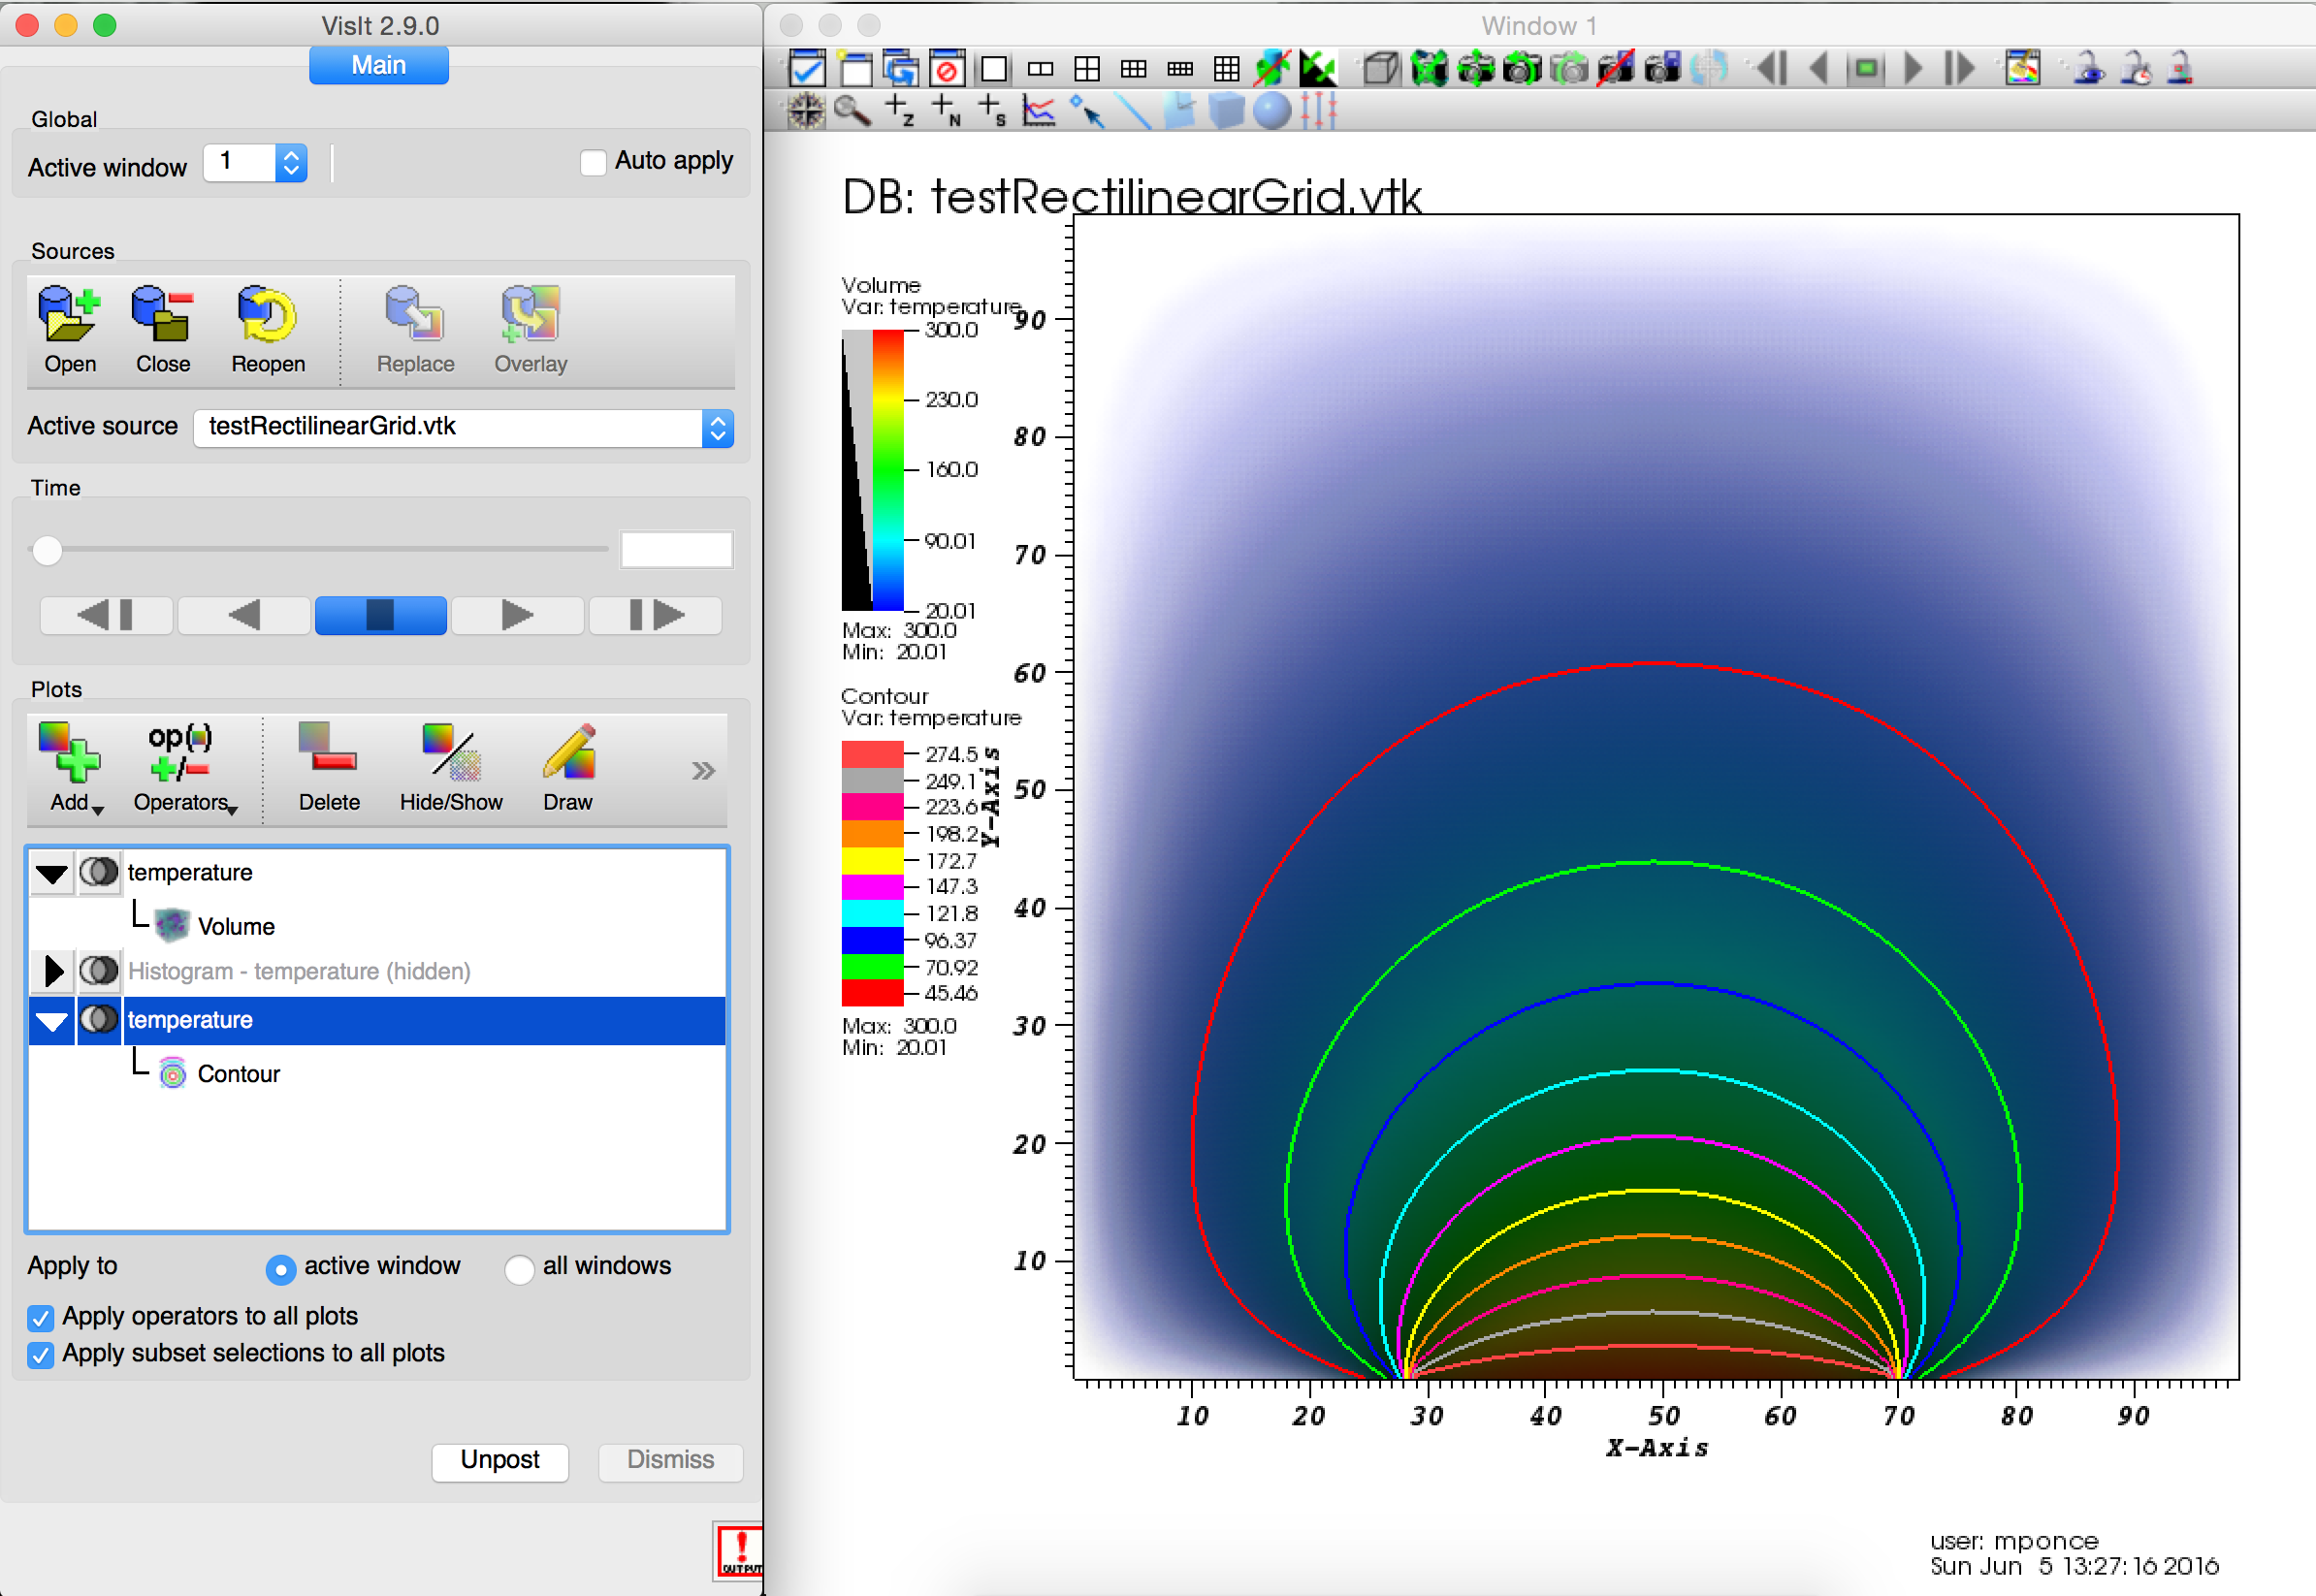
\includegraphics[width=.5\columnwidth]{figs/visit-handson/testRectilinearGrid_gui}
	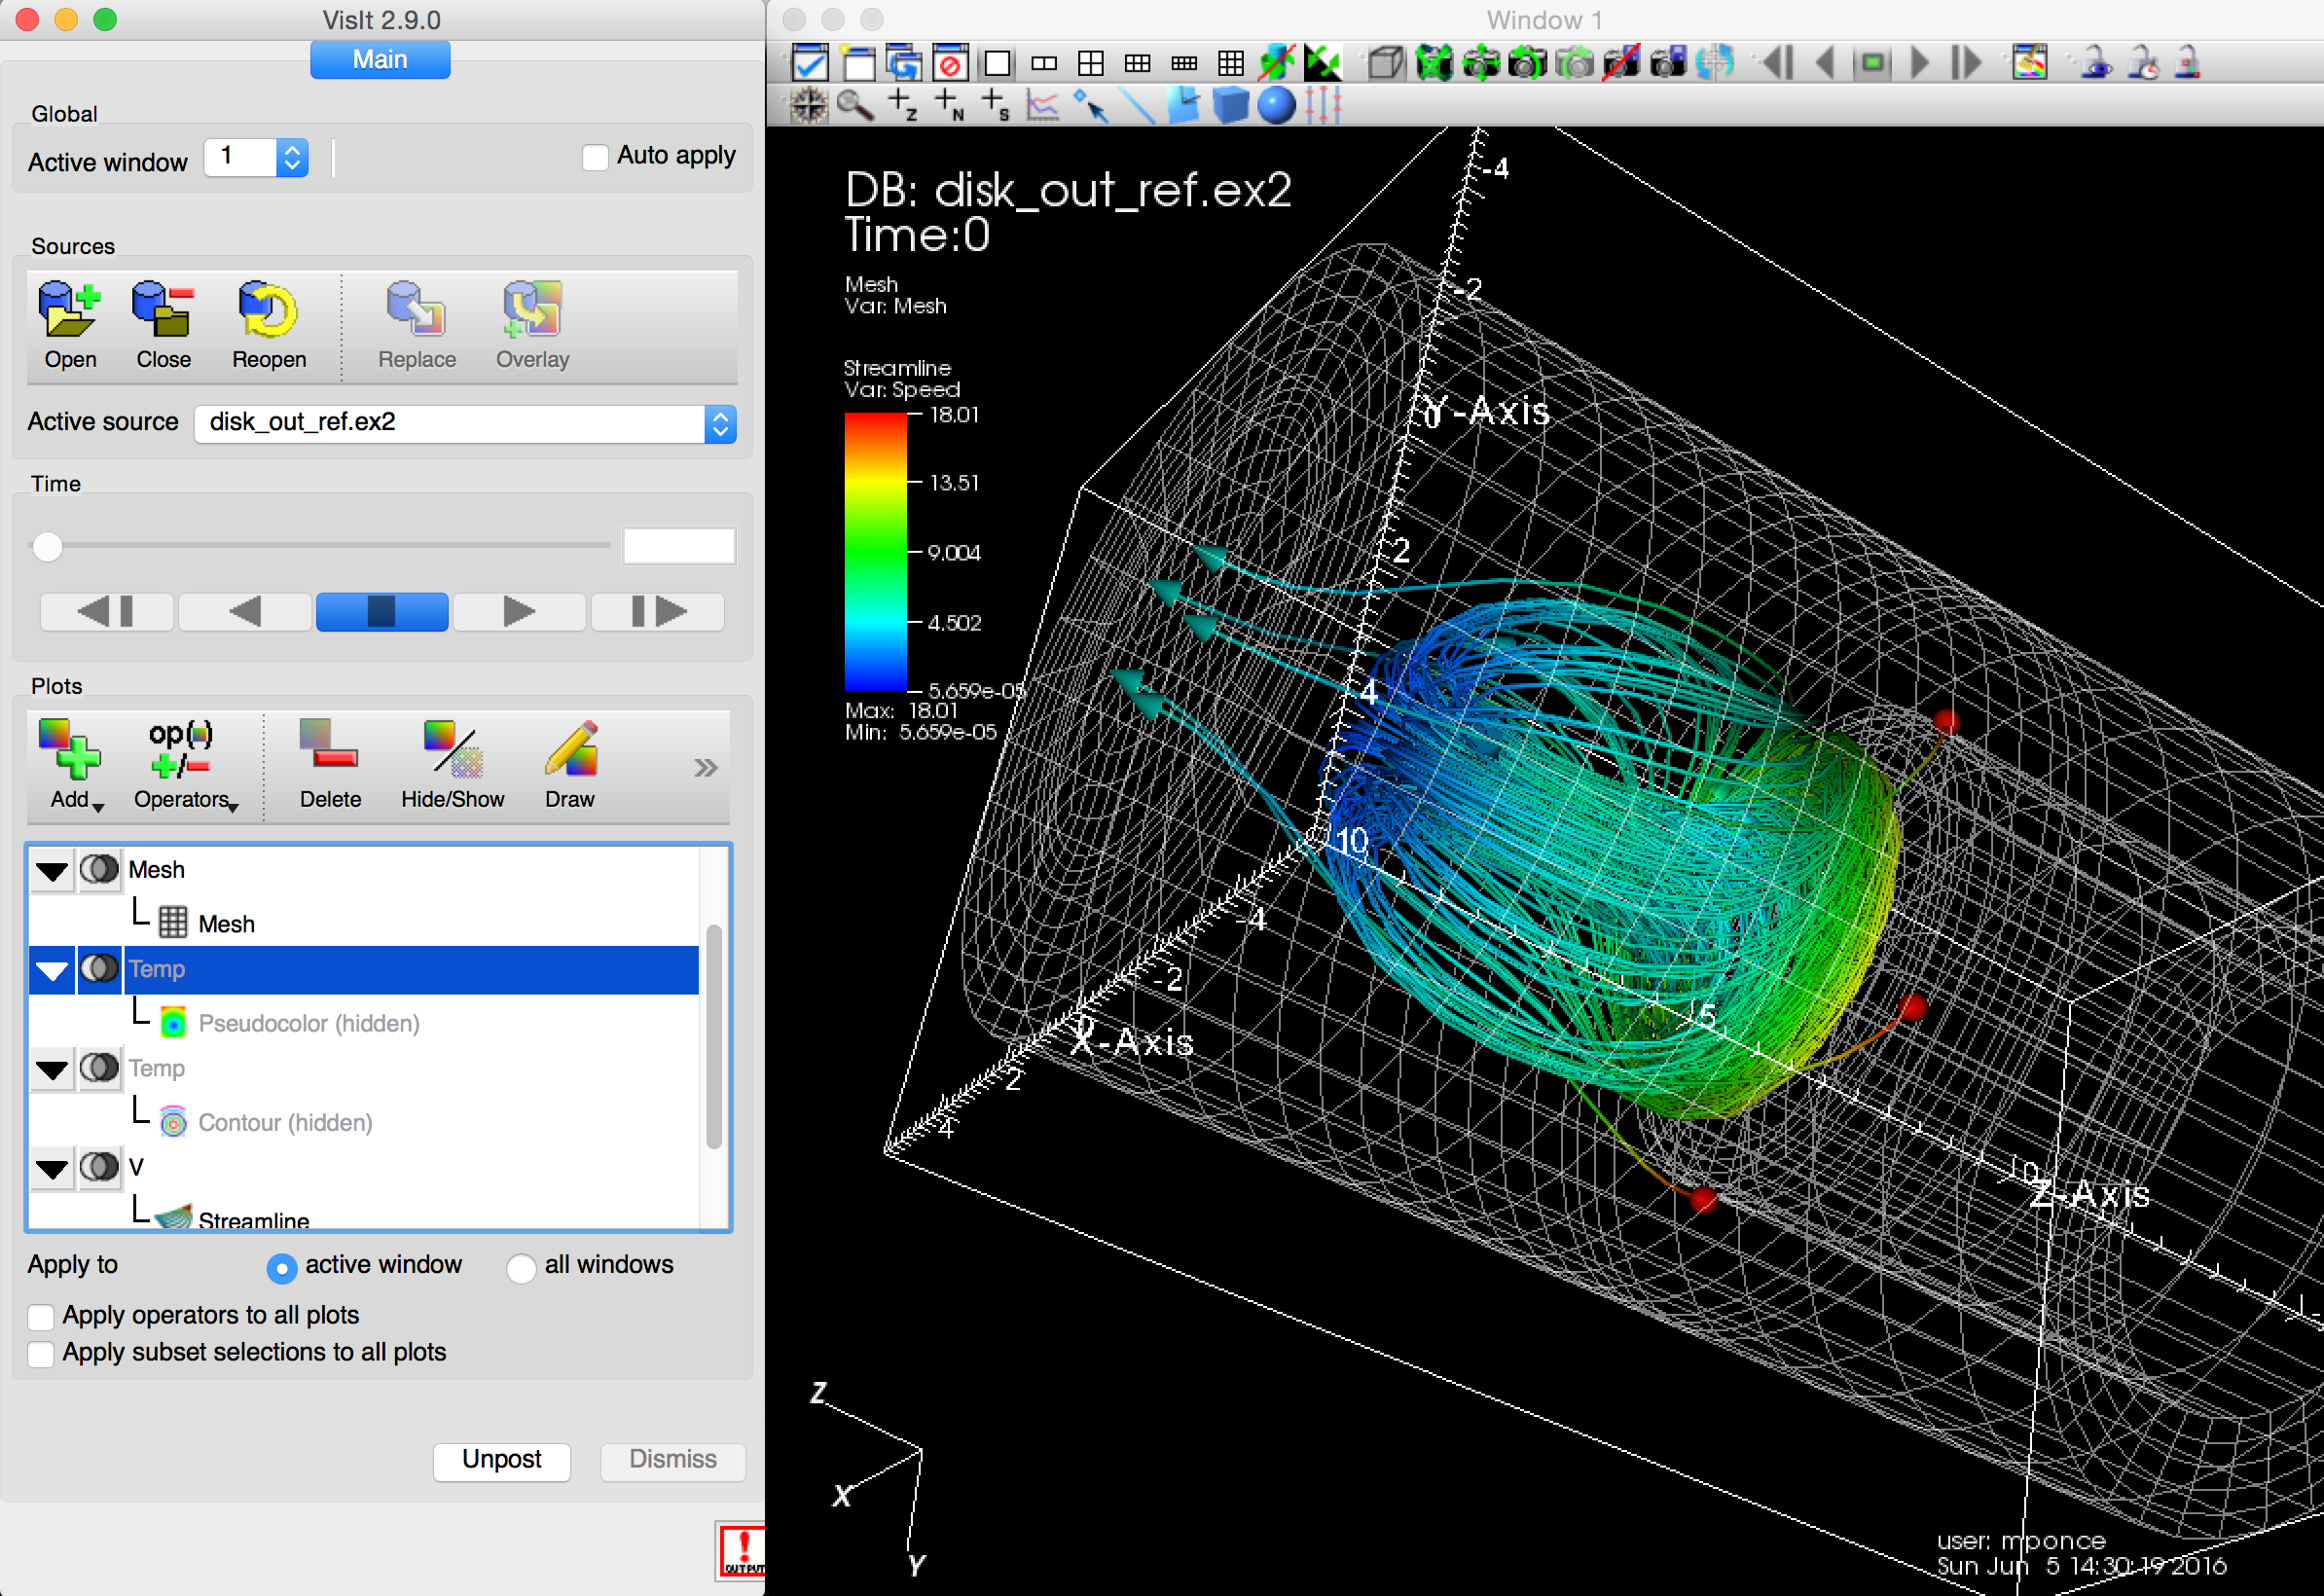
\includegraphics[width=.5\columnwidth]{figs/visit-handson/disk_out_ref-gui}

	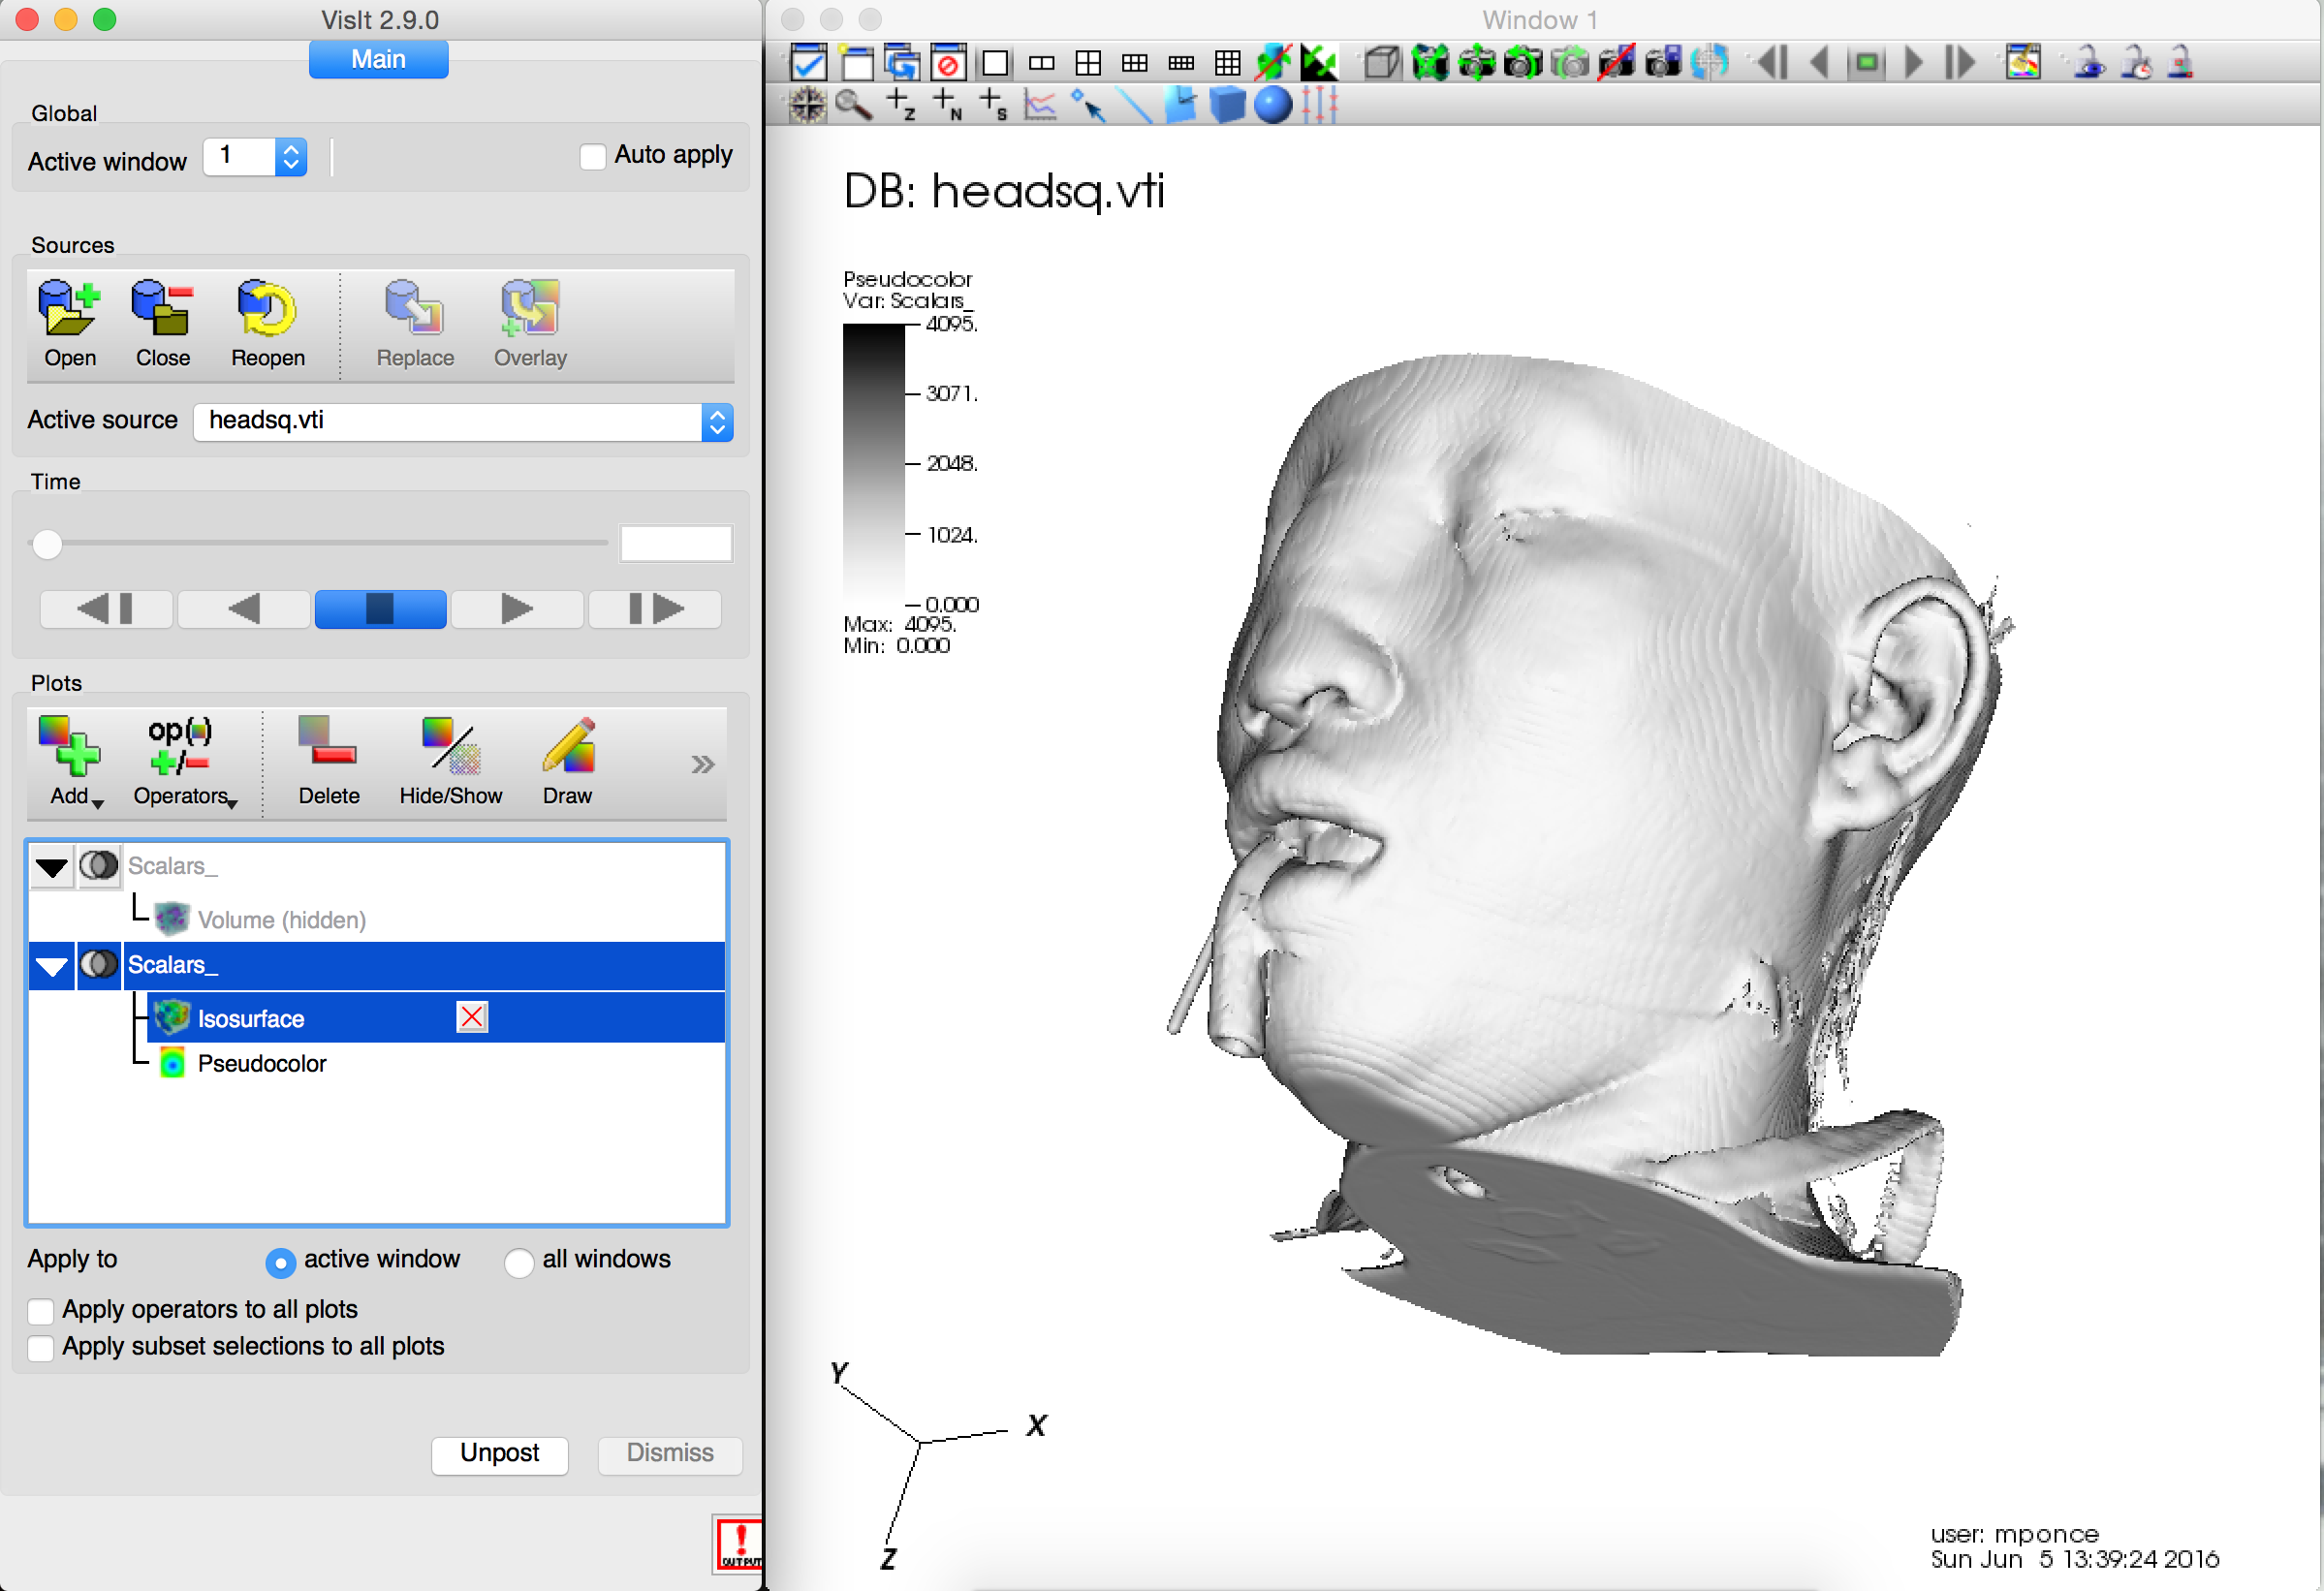
\includegraphics[width=.5\columnwidth]{figs/visit-handson/headsq_gui}
	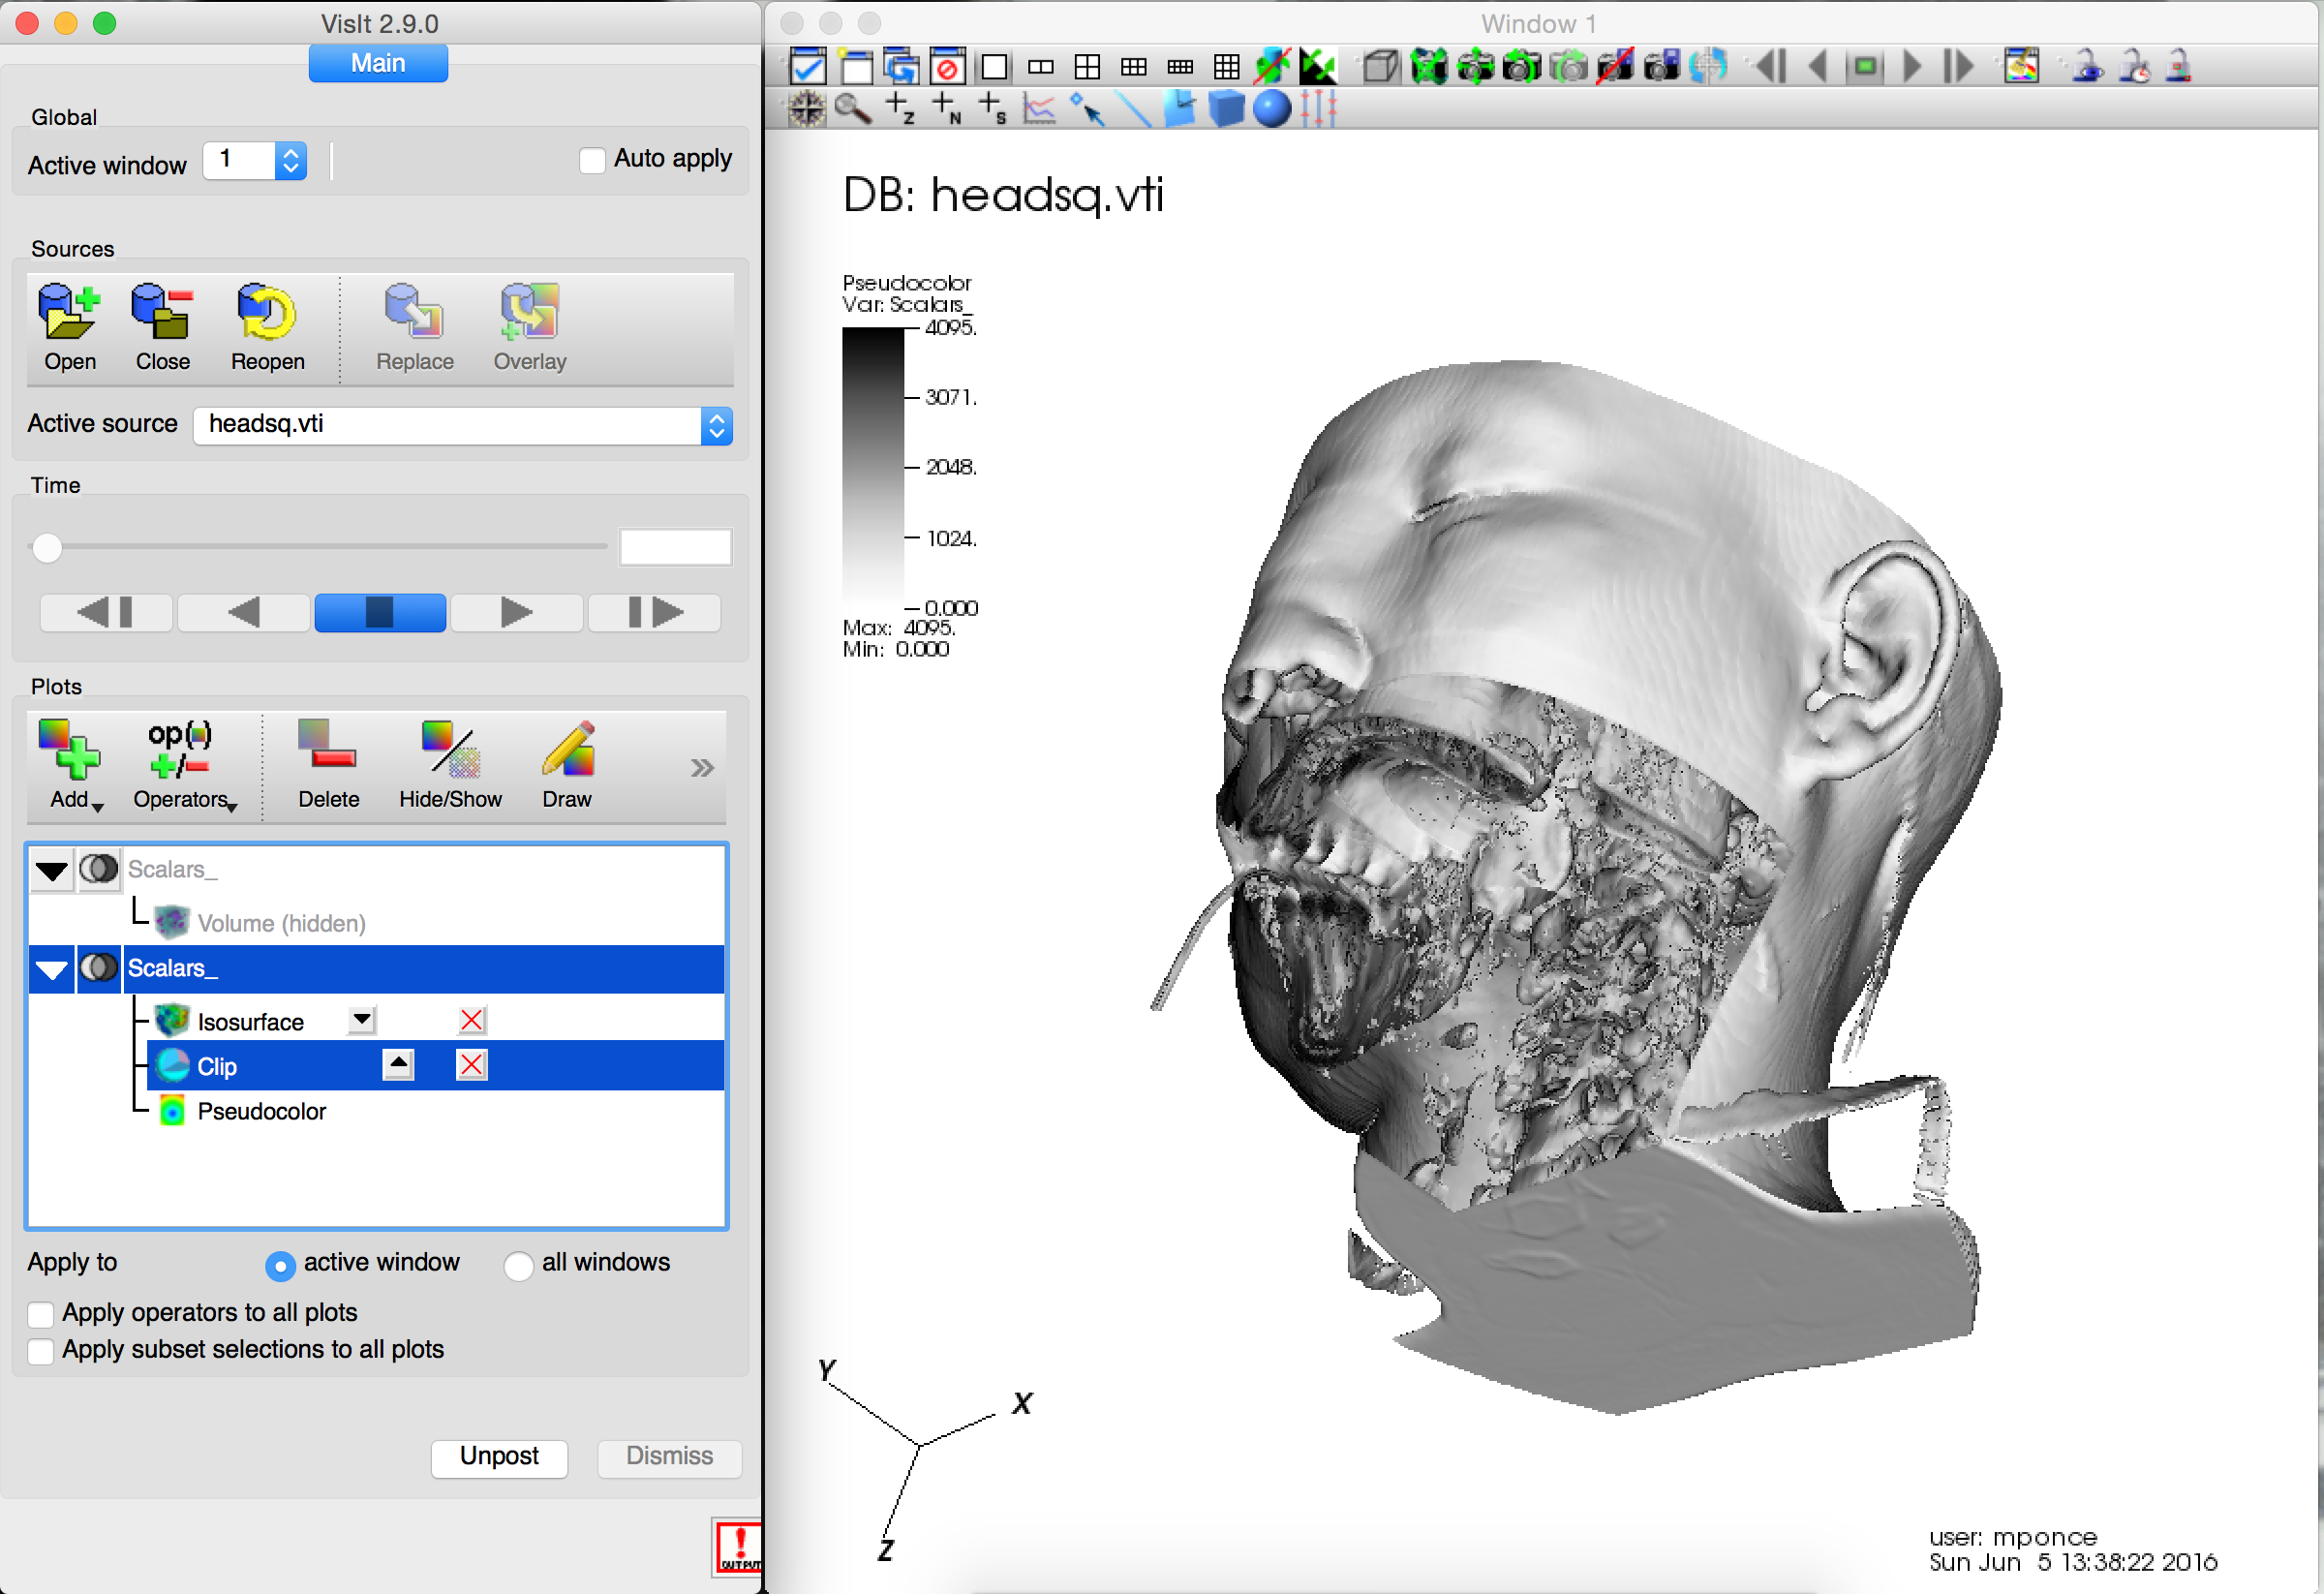
\includegraphics[width=.5\columnwidth]{figs/visit-handson/headsq-cut_gui}
\end{column}
\end{columns}
\end{frame}
%%%
\resetEnv
\basicEnv
